% =====================================================================
%  Presentation: Side-burnt document line completion (10 slides)
%  Compile with pdfLaTeX on Overleaf (upload this folder, compile main.tex).
% =====================================================================
\documentclass[aspectratio=169,11pt]{beamer}
\usetheme[progressbar=frametitle,numbering=fraction]{metropolis}
\usepackage[T1]{fontenc}
\usepackage[utf8]{inputenc}
\usepackage{booktabs}
\usepackage{tikz}
\usetikzlibrary{arrows.meta,positioning}
\graphicspath{{figures/}}

\definecolor{ink}{HTML}{1C232C}
\definecolor{burn}{HTML}{C2501F}
\definecolor{paper}{HTML}{F6F3EC}
\definecolor{tblue}{HTML}{2A6FC4}
\setbeamercolor{frametitle}{bg=ink,fg=paper}
\setbeamercolor{progress bar}{fg=burn,bg=burn!25}
\setbeamercolor{alerted text}{fg=burn}
\setbeamercolor{title separator}{fg=burn}
\setbeamercolor{background canvas}{bg=paper}
\setbeamercolor{block title}{bg=ink!10,fg=ink}
\setbeamercolor{block body}{bg=ink!4}
\setlength{\leftmargini}{1.2em}

\newcommand{\READ}{\textsc{read}}
\newcommand{\INF}{\textsc{inferred}}
\newcommand{\bignum}[1]{{\Large\bfseries\color{burn}#1}}

\title{Side-Burnt Document Line Completion}
\subtitle{Separating what the image can read from what context can only suggest}
\author{Praveen (AP23110010460) \quad Pranav (AP23110010457) \quad Samad (AP23110010747)}
\institute{Guide: Dr. Ravi Kant Kumar\\Department of Computer Science \& Engineering, SRM University-AP}
\date{UROP Project}

\begin{document}

% 1 -------------------------------------------------------------------
\maketitle

% 2 -------------------------------------------------------------------
\begin{frame}{Problem and key idea}
\centering
\includegraphics[width=0.9\textwidth,height=0.34\textheight,keepaspectratio]{fig_pipeline.png}\\
\scriptsize (a) original page \quad (b) mask: legible (white), faded but visible (orange), charred (black) \quad (c) model input

\vspace{0.4em}
\raggedright\footnotesize
When a page burns from the side, every line loses its end. Restoring it mixes two different problems:
\begin{columns}[T]
\begin{column}{0.48\textwidth}
\begin{block}{\READ\ (faded but visible)}
Strokes are still in the image. This is \textbf{recognition}: one right answer, and the image
is the evidence.
\end{block}
\end{column}
\begin{column}{0.48\textwidth}
\begin{block}{\INF\ (burnt away)}
Nothing is left in the image. This is \textbf{guessing} from context: many plausible answers.
\end{block}
\end{column}
\end{columns}

\vspace{0.3em}
Existing systems report one accuracy for both. \alert{\textbf{We score them separately}}, so
reading cannot hide guessing.
\end{frame}

% 3 -------------------------------------------------------------------
\begin{frame}{Methodology: synthetic data with exact labels}
\footnotesize
\begin{columns}[T]
\begin{column}{0.56\textwidth}
\begin{itemize}
\item 57 Project Gutenberg books, split \textbf{by book}: test text is never seen in training
\item Pages at $1024\times1024$ px in 16 fonts, with random size, margins, spacing, paper and
ink; indents, justification and hyphenation
\item Random burn: jagged edge (15--30\% of the width), fade band of 30--80\,px, scorch halo,
texture, blur, JPEG
\item Burn opacity: $\alpha(x,y)=\operatorname{clip}\!\left(\frac{x-(b(y)-T)}{T},0,1\right)^{\gamma}$
\item Labels per character: prefix if $\alpha<0.5$; \READ\ if $0.5\le\alpha<0.8$; \INF\ otherwise
\item Model input: the surviving text plus a $128\times256$ crop of the burn edge
\end{itemize}
\end{column}
\begin{column}{0.4\textwidth}
\centering
\begin{tabular}{@{}lrr@{}}
\toprule
Split & Books & Lines\\
\midrule
Train & 47 & 98{,}176\\
Val & 4 & 3{,}961\\
Test & 6 & 6{,}145\\
\bottomrule
\end{tabular}

\vspace{0.8em}
\includegraphics[width=\textwidth,height=0.3\textheight,keepaspectratio]{fig_line_zoom.png}\\
\scriptsize One labelled line: prefix, \READ\ (orange), \INF
\end{column}
\end{columns}
\end{frame}

% 4 -------------------------------------------------------------------
\begin{frame}{Methodology: model}
\centering
\resizebox{0.78\textwidth}{!}{%
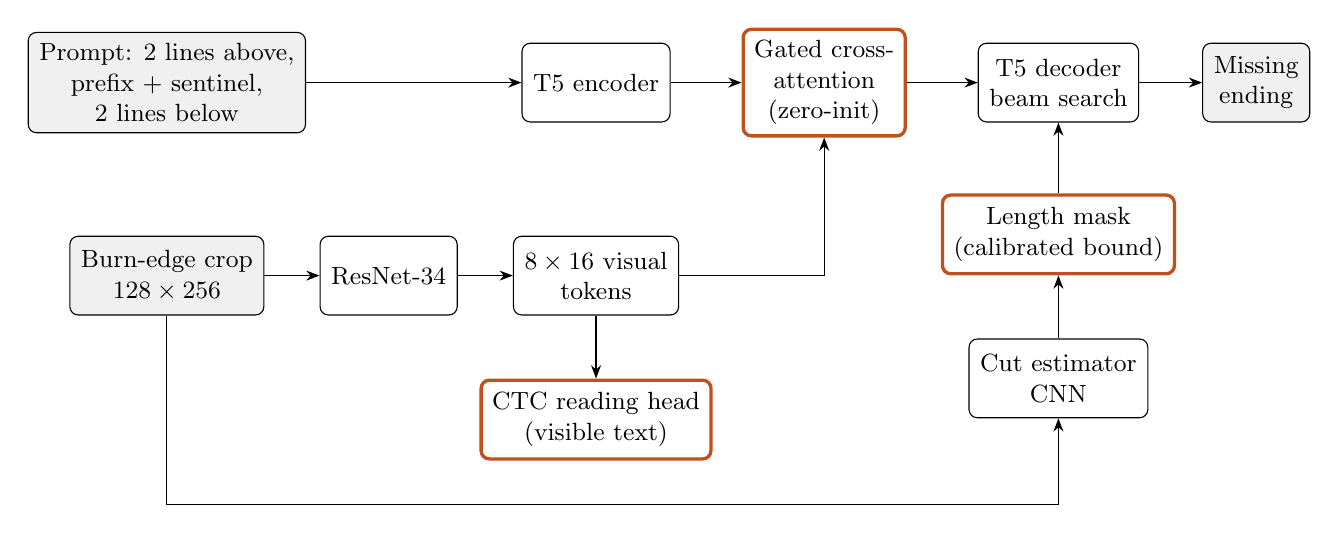
\begin{tikzpicture}[font=\small,>=Stealth,
  box/.style={draw,rounded corners=3pt,align=center,minimum height=1.0cm,inner sep=4pt,fill=white},
  io/.style={box,fill=black!6},
  ours/.style={box,draw=burn,very thick}]
\node[io] (crop) {Burn-edge crop\\$128\times256$};
\node[box,right=0.7cm of crop] (resnet) {ResNet-34};
\node[box,right=0.7cm of resnet] (tok) {$8\times16$ visual\\tokens};
\node[ours,below=0.8cm of tok] (ctc) {CTC reading head\\(visible text)};
\node[io,above=1.3cm of crop] (prompt) {Prompt: 2 lines above,\\prefix + sentinel,\\2 lines below};
\node[box] (enc) at (prompt -| tok) {T5 encoder};
\node[ours,right=0.9cm of enc] (fuse) {Gated cross-\\attention\\(zero-init)};
\node[box,right=0.9cm of fuse] (dec) {T5 decoder\\beam search};
\node[ours,below=0.9cm of dec] (bud) {Length mask\\(calibrated bound)};
\node[box,below=0.8cm of bud] (cut) {Cut estimator\\CNN};
\node[io,right=0.8cm of dec] (out) {Missing\\ending};
\draw[->] (crop) -- (resnet); \draw[->] (resnet) -- (tok);
\draw[->] (tok) -- (ctc);
\draw[->] (prompt) -- (enc); \draw[->] (enc) -- (fuse);
\draw[->] (tok.east) -| (fuse.south);
\draw[->] (fuse) -- (dec); \draw[->] (dec) -- (out);
\draw[->] (cut) -- (bud); \draw[->] (bud) -- (dec);
\draw[->] (crop.south) |- ++(0,-2.4) -| (cut.south);
\end{tikzpicture}}

\raggedright\footnotesize
\begin{itemize}
\item \textbf{T5} (60\,M / 220\,M) encodes the surrounding lines; its span-filling pretraining matches the task.
\item \textbf{Gated fusion}: $h' = h + \tanh(g)\,\mathrm{MHA}(h,V,V)$, $g=0$ at start, so the image is added only as it helps.
\item \textbf{CTC head} reads the visible strokes. Loss:
$\mathcal{L}=\mathcal{L}_{\text{gen}}+0.3\,\mathcal{L}_{\text{CTC}}+0.2\,\mathcal{L}_{\text{con}}$
(contrastive only on \READ\ characters). \textcolor{burn}{\textbf{Orange}} = our additions.
\end{itemize}
\end{frame}

% 5 -------------------------------------------------------------------
\begin{frame}{Methodology: length bound and evaluation}
\footnotesize
\begin{columns}[T]
\begin{column}{0.5\textwidth}
\textbf{Keeping guesses inside the burnt space}
\begin{itemize}
\item Estimate $\hat n$ = gap to the right margin / mean glyph width
\item The old rule cut off 7.6\% of \emph{correct} endings, yet let models run on
\item A small CNN finds the cut (error 0.96\,px, was 7.3\,px)
\item Upper bound $u = 1.139\,\hat n + 1$, calibrated so 99\% of true endings fit
\item Beam search masks any token that would cross $u$
\end{itemize}
\vspace{0.3em}
\bignum{20\%$\rightarrow$2\%} endings too long\\
\bignum{0} outputs over the bound
\end{column}
\begin{column}{0.46\textwidth}
\textbf{Evaluation protocol}
\begin{itemize}
\item 6{,}145 test lines from 6 unseen books
\item \READ\ accuracy: prediction starts with exactly the visible characters
\item \INF\ CER: character error rate on the burnt part
\item Also CER, exact match, top-5, AUROC and ECE
\item Compared: text-only model, image ablations, and an external TrOCR + Qwen2.5-1.5B baseline
\item Same beam search ($k=5$) and bound for all; paired bootstrap tests
\end{itemize}
\end{column}
\end{columns}
\end{frame}

% 6 -------------------------------------------------------------------
\begin{frame}{Implementation}
\footnotesize
\begin{columns}[T]
\begin{column}{0.5\textwidth}
\textbf{Training}
\begin{itemize}
\item Stage 1: T5 frozen; vision, fusion and heads learn (1 epoch)
\item Stage 2: everything fine-tuned with per-group learning rates
\item bfloat16, batch 16; t5-small 5 epochs, t5-base 3 epochs
\item One RTX 4050 laptop GPU (6\,GB); PyTorch + Transformers
\end{itemize}
\end{column}
\begin{column}{0.46\textwidth}
\textbf{System}
\begin{itemize}
\item Burn detector finds 99.6\% of severed lines on a full page
\item FastAPI web demo: suggestions, alternatives, vision-only reading, length estimate
\item States that suggestions are hypotheses
\item 115 unit and integration tests
\end{itemize}
\end{column}
\end{columns}

\vspace{0.4em}
\centering
\includegraphics[width=0.48\textwidth,height=0.36\textheight,keepaspectratio]{fig_training.png}
\hfill
\includegraphics[width=0.44\textwidth,height=0.36\textheight,keepaspectratio]{fig_ui_demo.png}\\
\scriptsize Left: training curves. Right: the web demo on a held-out page.
\end{frame}

% 7 -------------------------------------------------------------------
\begin{frame}{Outcomes: the image reads, it does not recover burnt text}
\centering
\footnotesize
\begin{tabular}{@{}lcccc@{}}
\toprule
System (6{,}145 test lines) & \READ\ acc $\uparrow$ & \INF\ CER $\downarrow$ & CER $\downarrow$ & 1st word $\uparrow$\\
\midrule
Text only, t5-small & 0.232 & 0.815 & 0.775 & 16.6\%\\
\textbf{Ours, t5-small} & \textbf{0.700} & 0.768 & 0.699 & 40.1\%\\
Text only, t5-base & 0.361 & 0.741 & 0.702 & 29.3\%\\
\textbf{Ours, t5-base} & 0.660 & \textbf{0.717} & \textbf{0.656} & \textbf{41.8\%}\\
\bottomrule
\end{tabular}

\vspace{0.6em}
\raggedright
\begin{columns}[T]
\begin{column}{0.5\textwidth}
\textbf{Main result}
\begin{itemize}
\item The image raises \READ\ accuracy \alert{\textbf{0.23 $\rightarrow$ 0.70}}
\item The burnt part improves only a little
\item t5-base is the better guesser
\item All differences significant ($p<0.001$)
\end{itemize}
\end{column}
\begin{column}{0.46\textwidth}
\textbf{Ablation (\READ\ accuracy)}
\begin{itemize}
\item Real crop \textbf{0.70}, blank image \textbf{0.16}, another line's crop \textbf{0.07}
\item So the model reads \emph{this} line's strokes
\item Burnt part: same error with or without the image
\end{itemize}
\end{column}
\end{columns}
\end{frame}

% 8 -------------------------------------------------------------------
\begin{frame}{Outcomes: baseline and confidence}
\footnotesize
\begin{columns}[T]
\begin{column}{0.52\textwidth}
\textbf{vs.\ off-the-shelf OCR + 1.5B LLM}\\[0.3em]
\includegraphics[width=\textwidth,height=0.3\textheight,keepaspectratio]{fig_baseline.png}
\begin{itemize}
\item TrOCR + Qwen2.5-1.5B (7$\times$ larger), same length bound
\item \textbf{Reads as well}: \READ\ 0.66 vs 0.66
\item \alert{\textbf{Guesses far worse}}: \INF\ CER 0.95 vs 0.72; 38\% of its endings too long vs 2\%
\end{itemize}
\end{column}
\begin{column}{0.44\textwidth}
\textbf{Confidence you can trust}\\[0.5em]
\bignum{88\%} of the most confident quarter of first words are right (70\% text only)
\begin{itemize}
\item AUROC 0.87: confidence separates right from wrong
\item ECE 0.03: stated confidence matches real accuracy
\item The demo can show confident suggestions and flag the rest for a human
\end{itemize}
\end{column}
\end{columns}
\end{frame}

% 9 -------------------------------------------------------------------
\begin{frame}{Conclusion, limitations and next steps}
\footnotesize
\begin{itemize}
\item \textbf{The image reads} faded letters (\READ\ 0.23 $\rightarrow$ 0.70); \textbf{context
guesses} the burnt part; the calibrated bound was the largest gain on the guess.
\item Beats a 7$\times$ larger OCR + LLM pipeline on the burnt part, with calibrated confidence.
\end{itemize}
\begin{columns}[T]
\begin{column}{0.48\textwidth}
\textbf{Limitations}
\begin{itemize}
\item Synthetic burns only
\item Right-side burns of printed English text
\item Each model trained once
\item Exact matches rare (10\%): suggestions, not restoration
\end{itemize}
\end{column}
\begin{column}{0.48\textwidth}
\textbf{Next steps}
\begin{itemize}
\item Real burnt-paper test
\item Repeated runs (3 seeds)
\item OCR stage for photos
\item Stronger baselines (fine-tuned, 7B LLMs)
\end{itemize}
\end{column}
\end{columns}

\vspace{0.5em}
\centering
\alert{\textbf{The image reads. Context guesses. We keep them apart.}}
\end{frame}

% 10 ------------------------------------------------------------------
\begin{frame}[standout]
Thank you!\\[0.5em]
Questions?
\end{frame}

\end{document}
